\subsubsection{Seriel kommunikation}

\textbf{Devkit8000-PSoC Master:} \\

Som beskrevet i analysen for SPI (reference), blev denne protokol valgt pga. den kendskab gruppen allerede havde fra HAL øvelse 6 (reference). 
SPI device driveren fra denne øvelse blev benyttet som udgangspunkt til at lave en tilpasset driver, som kunne kommunikere med PSoC Master. 
Denne forbindelse viste sig dog at volde store problemer for gruppen, og det lykkedes ikke at få hverken sendt eller modtaget data med denne driver.\\

Det blev herefter besluttes at der ikke skulle bruges mere tid på selv at lave en driver, og istedet benytte en SPI device driver som var udleveret fra skolen.
Dog var det blot den binære fil som var tilgængelig, hvilket betød at der ikke var adgang til source-koden. Dette gjorde at gruppen ikke kunne tilpasse driveren,
og alt information omkring opsætningen for SPI forbindelse måtte udledes fra det PSoC-Creator program som medfulgte. 

\begin{figure}[H]
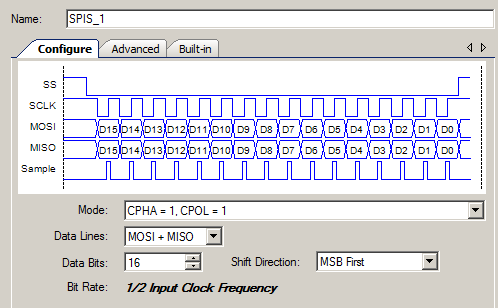
\includegraphics[scale=0.6]{tex/Design/SPI/Clock_mode_SPI}
\caption{Opsætning for SPI forbindelse Devkit8000-PSoC Master}
\end{figure}

Ud fra figur xx, kan det aflæses at SPI clock mode er sat til CPHA = 1 og CPOL = 1, og bitsperword til 16 databits. Det PSoC program som var udleveret blev brugt
som skabelon for gruppens eget program til PSoC master, dog med nogle modifikationer. Især behandlingen af de databits som blev modtaget fra devkittet blev 
genbrugt, da der ikke kunne ændres på disse bits. Koden består dybest set at en interrupt service rutine (ISR), som kaldes hver gang
der modtages data fra devkittet. I ISR er der implementeret en switch, der sørger for at de rigtige metoder kaldes alt efter hvilke databits der modtages.
For mere information omkring koden for PSoC master henvises til bilag(navn på bilag). \\

\textbf{PSoC Master - PSoC Slave:} \\

Til SPI forbindelsen mellem PSoC Master og PSoc slave havde gruppen frie hænder til opsætte SPI. Her blev clock mode valgt til CHPA = 0 og CPOL = 0, og 
bitsperword til 8. Grunden til der kun bliver sendt 8 bits her, er at det er tilstrækkeligt til den simple form for kommunikation der er mellem PSoc enhederne.
8 databits ville også have været fint for Devkit-PSoC forbindelsen, men som tidligere nævnt kunne det ikke ændres da der ikke var adgang til SPI device driveren
på Devkit8000. Clock mode er ændret til default værdien fra PSoC-Creator, og har ikke nogen betydning for kommunikationen så længe begge PSoC enheder har samme
clock mode. Koden for PSoC Slave indeholder ligesom i PSoC master en switch der alt efter de modtagne databits kalder metoder til udførsel af diverse opgaver. 
For mere information omkring koden for PSoC slave henvises til bilag(navn på bilag).   


